\section{实验}\label{sec:exp}
\subsection{实验设置}
我们从StrategyQA、MMLU-Hard和TruthfulQA各使用150道留出题。每个条件包含5个Agent和3轮同步审议，主后端为DeepSeek-V3~\cite{deepseek2024v3}。确认性实验包含$450\times3=1{,}350$条问题--条件记录和20,250个Agent-round。三种规则的问题、Seed、面板、轮数和聚合方式均配对，只有公开合同改变。最终决策取第三轮明确结论的多数票。

主要结果是高资源行动率（\textsc{AEIC}与\textsc{Verify}占比）和问题级准确率；同时报告每Agent-round Token、采集完整性和分域效应。配对二元结果采用精确McNemar检验，并在注册比较族内进行Holm校正。图~\ref{fig:evidence}概括识别逻辑和证据层级。
\begin{figure}[t]\centering
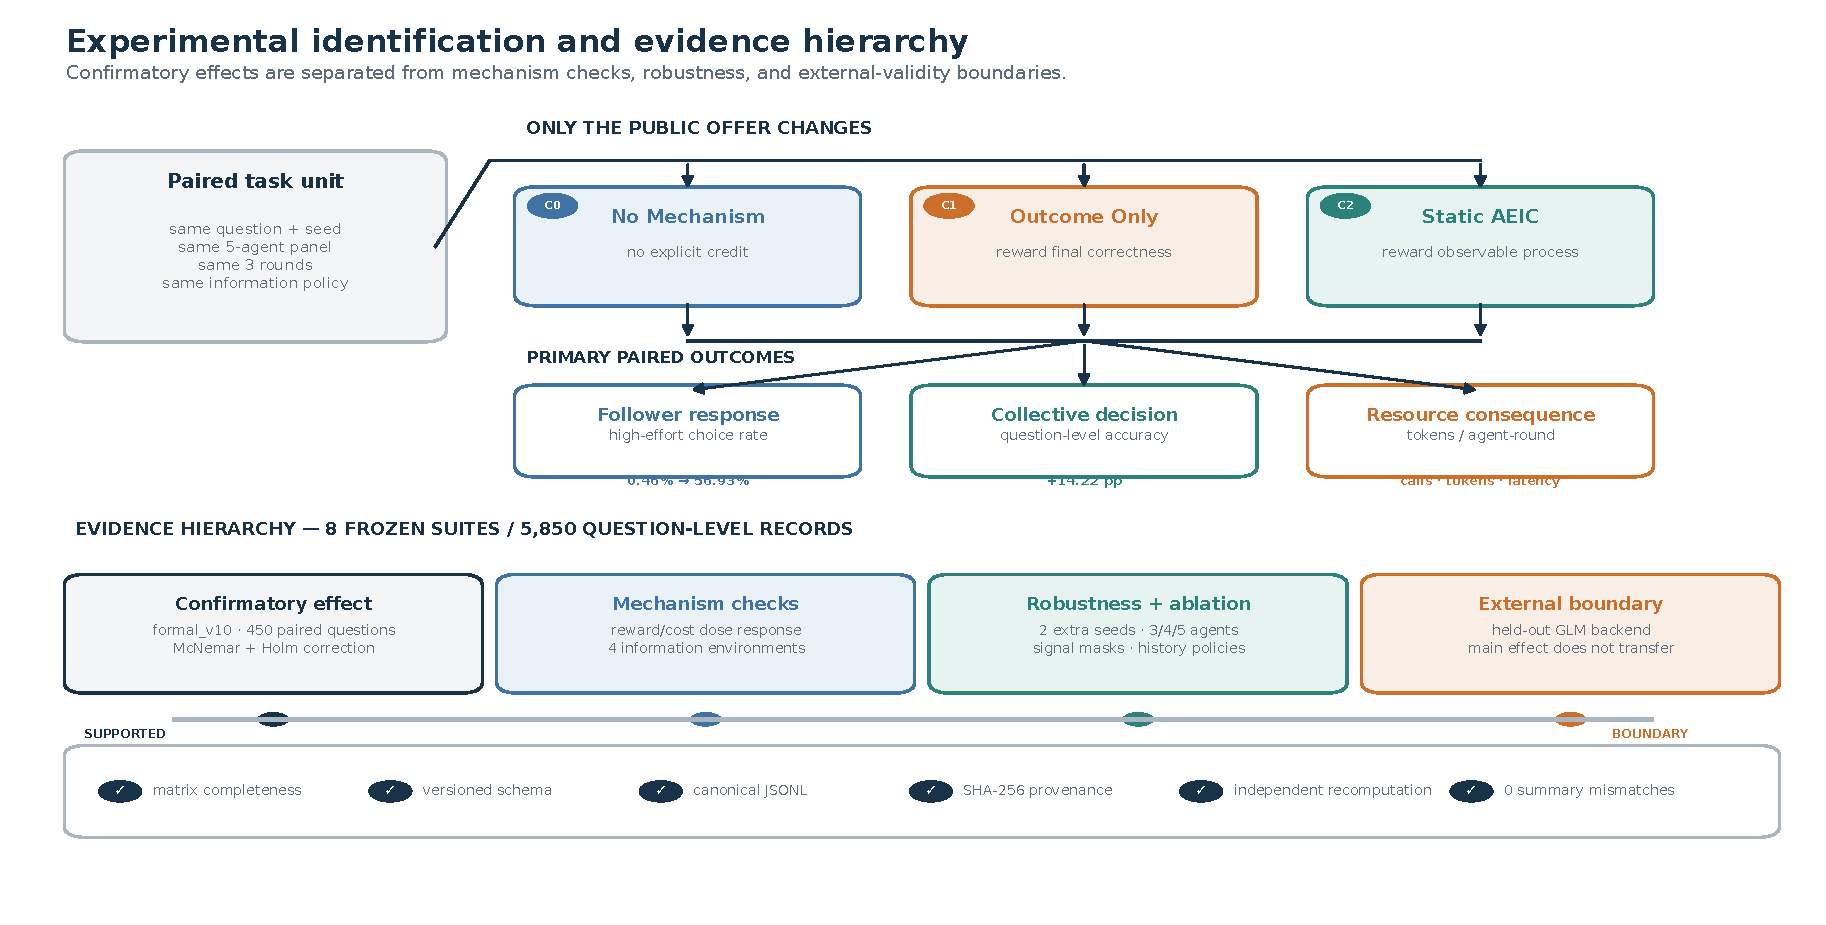
\includegraphics[width=\textwidth]{../figures/fig3_experimental_design.pdf}
\caption{实验识别与证据层级。配对条件隔离公开规则，八组冻结实验覆盖确认、机制检验、稳健性、消融与不迁移边界。}\label{fig:evidence}\end{figure}

\subsection{确认性追随者响应检验}
\begin{table}[t]
\caption{450道问题上的确认性配对检验。高资源行动在每种规则的6,750个Agent-round上测量。}\label{tab:main}
\centering\small
\begin{tabular}{@{}lccc@{}}\toprule
规则 & 高资源行动 & 准确率 & Token/Agent-round \\\midrule
No Mechanism & 0.46\% & 68.00\% & 663.3 \\
Outcome Only & 3.08\% & 67.33\% & 689.2 \\
Static AEIC & \textbf{56.93\%} & \textbf{82.22\%} & 808.8 \\\bottomrule
\end{tabular}\end{table}

Static AEIC同时改变追随者行为和集体决策（表~\ref{tab:main}；图~\ref{fig:formal}）。高资源行动率增加56.47个百分点；准确率增加14.22个百分点，相对No Mechanism有78道题由错变对、14道由对变错（Holm校正McNemar $p=1.23\times10^{-11}$）。每Agent-round额外145.5 Token与更完整工作的资源成本一致。

Outcome Only只将高资源行动率提高2.62个百分点，准确率变化$-0.67$个百分点（27道纠正、24道受损；$p=0.780$）。因此主效应不能概括为“告诉模型存在奖励”；区别在于规则是否提供追随者可通过生产过程满足的局部标准。
\begin{figure}[t]\centering
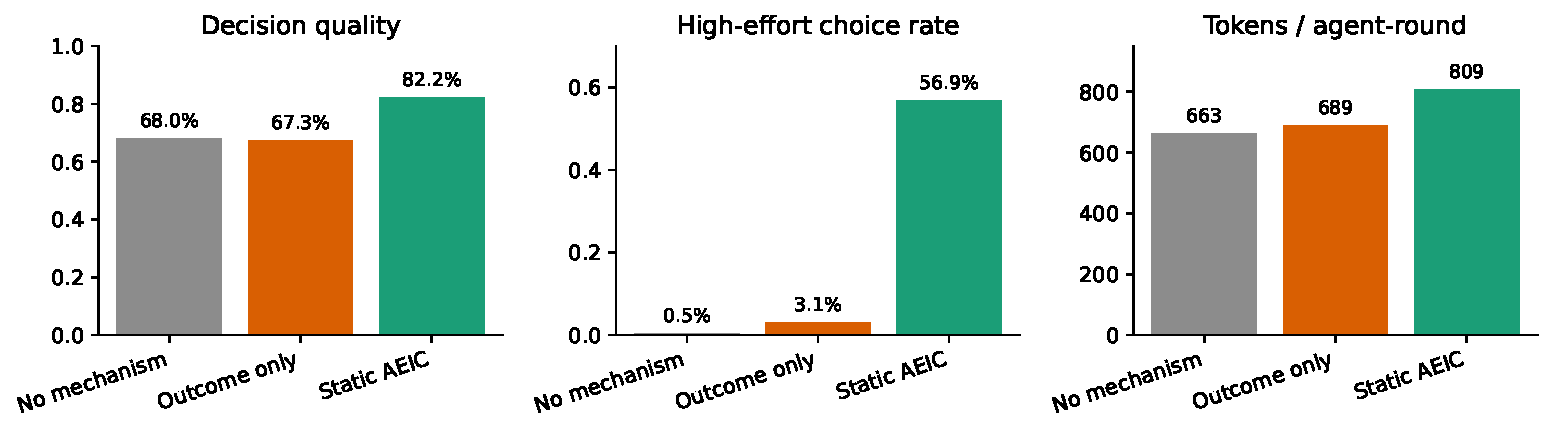
\includegraphics[width=\columnwidth]{../en/figures/fig1_formal_mechanism.pdf}
\caption{正式配对比较。基于AEIC接口的公开过程合同改变资源行动；合同、执行提示与分级资源路由的联合配置改善最终准确率，仅结果奖励没有改善准确率。}\label{fig:formal}\end{figure}

增益存在分域异质性：StrategyQA为$+4.0$、MMLU-Hard为$+20.0$、TruthfulQA为$+18.7$个百分点；对应高资源行动增益为43.5、73.7和52.2个百分点。因此总体效应不是任务无关常数。

从题目级流向看，Static AEIC相对No Mechanism产生78次错$\rightarrow$对和14次对$\rightarrow$错，净纠正64题。每题平均增加2,182 Token和0.80次调用，相当于每净纠正一题增加15,343 Token和5.64次调用。该结果正面呈现了质量收益的资源代价，而不是把准确率改善表述为免费收益。

\subsection{报告接口与机制成分分解}
为区分AEIC报告接口与合同执行效果，我们在90道配对问题上固定模型、调用次数和最大Token预算，比较自由文本、通用“分析--答案”结构和AEIC。三者准确率分别为72.22\%、82.22\%和85.56\%；AEIC相对自由文本提高13.33个百分点（Holm $p=0.00836$），但相对通用结构仅提高3.33个百分点（$p=0.453$）。因此AEIC的已证实作用是提供统一、可解析、可结算的语义接口；当前结果不支持其格式具有独立于一般结构化输出的准确率优势。

进一步在60道配对问题上固定DeepSeek后端，比较无合同固定资源、有合同固定资源、无合同匹配算力和完整机制。其高资源行动率分别为14.44\%、81.11\%、17.78\%和81.11\%，准确率分别为85.00\%、88.33\%、86.67\%和91.67\%。完整机制相对匹配算力将高资源行动提高63.33个百分点（$p=2.82\times10^{-33}$），实际Token差异不显著（$p=0.229$），说明行为响应不能由机械增加计算量解释。准确率差为$+5$个百分点，但仅有3次错$\rightarrow$对、0次对$\rightarrow$错（$p=0.25$），故只作为方向性成分证据。

\subsection{奖励--成本响应}
在每个任务域，奖励从0.05增至0.2和0.5时高资源行动单调不减；成本倍率从0.5增至1.0和1.5时单调不增（图~\ref{fig:boundary}）。冻结极值汇总中，高资源行动随奖励由49.42\%升至72.84\%，随成本由69.51\%降至53.78\%。中点来自同域开发观察，因此该实验是方向性机制检查而非第二个确认性效应。
\begin{figure}[t]\centering
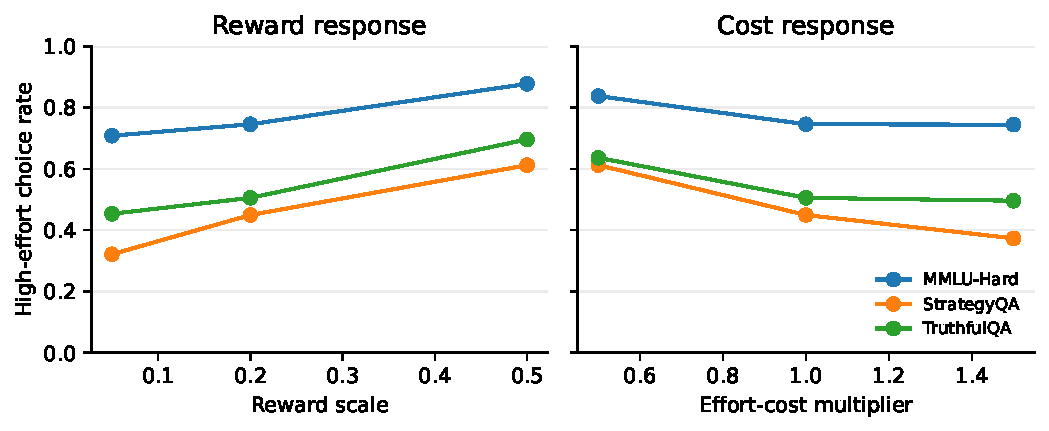
\includegraphics[width=\columnwidth]{../en/figures/fig2_incentive_response.pdf}
\caption{对公开合同的方向性响应：奖励提高时资源行动上升，行动成本提高时下降。}\label{fig:boundary}\end{figure}

\subsection{受控信息环境}
我们只改变第一轮后可见的同伴信息：新增证据、无证据多数立场、带复制压力的完整报告或立场相反证据。四类环境中，Static AEIC将汇总高资源行动率从0.86\%提高到49.41\%；各条件下为40.89\%--59.33\%，无机制时为0.44\%--1.47\%（图~\ref{fig:info}）。这说明接口在不同信息结构下仍有行为作用，但不证明每种信息干预都改善准确率或消除模仿。
\begin{figure}[t]\centering
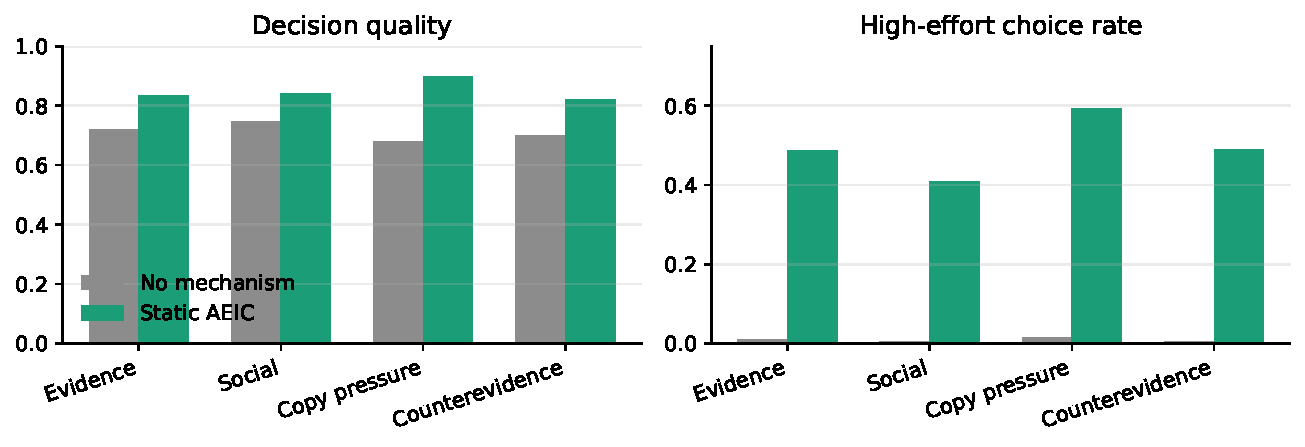
\includegraphics[width=\columnwidth]{../en/figures/fig3_information_conditions.pdf}
\caption{受控信息环境中的高资源行动。Static AEIC在四种设置中均改变行为。}\label{fig:info}\end{figure}

\subsection{稳健性、消融与外部有效性}
两个额外Seed复现主方向：Static AEIC准确率85.67\%，无机制71.00\%（$+14.67$个百分点；Holm校正$p=2.40\times10^{-9}$）。3、4、5 Agent条件下准确率为87.33\%--88.67\%。信号遮蔽和历史策略变体只限定当前实现，并不证明每个字段独立必要；移除字段会改变后端对整个合同的理解，因此属于干预消融而非模块化证明。
\begin{figure}[t]\centering
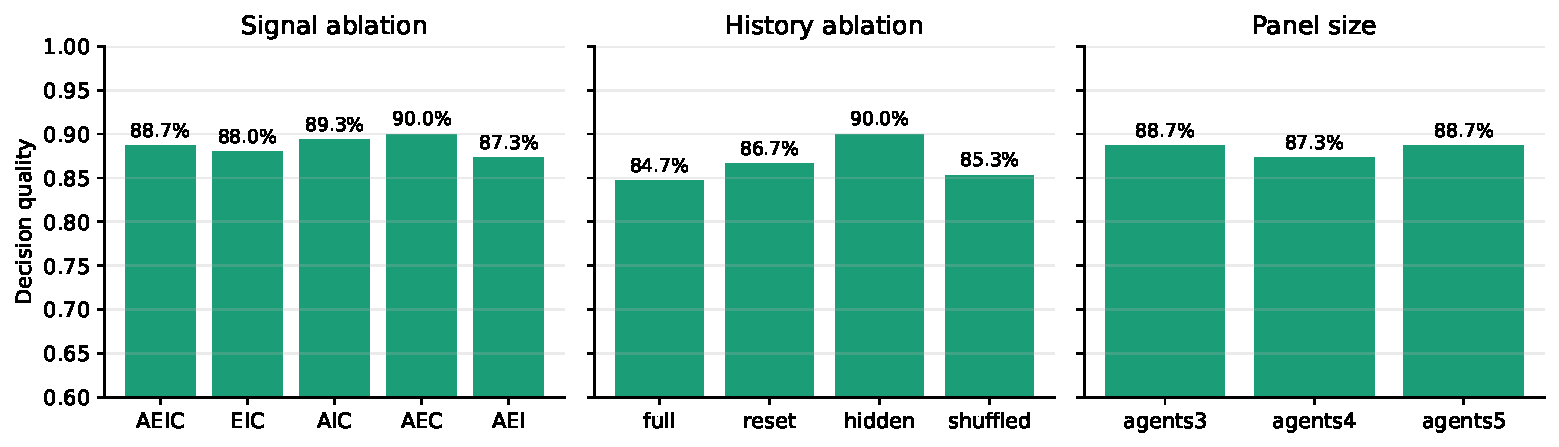
\includegraphics[width=\columnwidth]{../en/figures/fig4_ablations_robustness.pdf}
\caption{信号、历史、Seed与面板规模稳健性。组件变体是描述性边界。}\label{fig:robust}\end{figure}

留出GLM后端给出最强边界。Static AEIC仅将高资源行动率从0.58\%变为0.93\%（$p=0.134$），准确率为69.33\%，而无机制为70.67\%（Holm校正$p=0.791$）。相同文字和数值并不跨模型定义同一有效合同。当前公开过程合同仅在已测试主后端上得到实验支持，不是普适校准的激励语言。

\subsection{完整性与可复现性}
八组冻结实验的5,850条预期问题级记录全部存在；新增报告接口与机制拆解分别包含270和240条正式记录，总计6,360条。各冻结组通过Schema和路由验证，独立复算包与摘要无差异；机制拆解240条记录同样通过完整性检查。确认性数据中API终止失败为零、成本日志完整；少量解析失败经重试且保留在尝试日志。Manifest保存标准哈希，防止分析记录被静默替换。
